\chapter{Implementierung}

Die Implementierung beschreibt ganz grundlegende technische Details der Umsetzung. Das kann von konkreten Entscheidungen, wie der Wahl einer bestimmten Programmiersprache oder bestimmter Software-Bibliotheken, bis hin zu Auszügen aus dem Programmcode gehen.

Typischer Umfang der Implementierung: 5-10 Seiten BA, 15-20 Seiten MA.

\section{Learning Managment System}
Viele LMS sind auf dem Markt angeboten. Ein geeignete Plattform für das Projekt wird ausgewahlt. Auf diesem LMS wird ein Unterricht über Infusionsvorbereitung gestaltet. Paar Lernmethoden beispielsweise VR Übung werden in dem Unterricht eingesetzt. 

 \subsection{Applikation Auswahl}
 Laut Capterra stehen mehr als 400 LMS mit Web Applikation zu Verfügung. Jede LMS hat eigne Merkmale. Moodle wird als die LMS Plattform in diesem Projekt eingesetzt.
 
 Der größte Vorteil von Moodle für das Projekt ist, dass Moodle eine kostenlos open source LMS Plattform ist. Das heißt, dass es möglich ist, die Moodle gratis auf eigenem Server zu installieren, mit eigener Datenbank zu verbinden und nach eigenen Anforderungen anzupassen.
 
 Durch die vielfältige Aktivitäten in Moodle beispielsweise Aufgabe, Befragung, Test usw. können unterschiedliche Lernmethode eingesetzt werden. Mit dem Plugin System kann man selbst mit PHP eigene Aktivität schreiben und in Moodle integrieren, dadurch der zweite und dritte Form der Verbindung zwischen LMS und WebVR, die in Kapitel Konzeption genannt sind, implementiert werden können.
 
 In Moodle können auch Arbeitsmaterialien wie Buch, Datei, Link usw. angeboten werden. Bei diesem Projekt wird der Benutzer durch den URLs in Moodle zu der WebVR Applikation geleitet, wie die erste Form, die in Konzeption beschrieben wird. 
 
 \subsection{Unterricht}
 Bei dem Unterricht Infusion Vorbereitung werden fünf Arbeitsmaterialien (drei Links, eine Datei und ein Textseite) und eine Aktivität eingesetzt. Die drei Links leiten jeweils auf einer Erklärung über Infusionsvorbereitung in Text, einer Erzählung über 5-R-Regel in Text und einem Video über Infusionsvorbereitung auf Youtube um. Die Datei ist ein Diagramm, damit der Ablauf der Vorbereitung einer Infusion graphisch dargestellt wird.
 
 Die Textseite ist die Zugang der praktische Übung in VR Umgebung. Die Methoden der Interaktion für unterschiedlichen Geräten werden zuerst informiert. Danach wird der Ablauf mit dem Diagramm noch einmal wiederholt. Und die acht Abschnitte in der Übung werden bezeichnet. Zum Abschluss werden acht Links aufgelistet, die auf dem entsprechenden Abschnitt in der VR Übung umleiten.
 
 Am Ende des Unterrichtes wird die Aktivität Test angeboten. Dadurch wird das Effekt des Lernens überprüft. Und das Ergebnis wird in Moodle gespeichert.
 
 Die VR Übung und der Test sind wiederholbar, um die Lernenden zu helfen, die Fertigkeit richtig zu beherrschen.
 
 image: Unterricht und Textseite .........
 
\section{WebVR Übung}
Die Implementierung der WebVR Übung ist der Schwerpunkt dieses Projektes. .........

 \subsection{Framework Auswahl}
 
 Um die Ziele dieses Projektes zu erreichen, muss das ausgewählte Framework folgende Anforderungen erfüllen:
 
 \begin{enumerate}
     \item Das Projekt kann gut mit LMS kommunizieren. Die Kommunikation kann durch URL oder Datenbank realisiert werden.
     \item Das Framework kann unterschiedlichen Geräte unterstützen, z.B. PC, Smartphone und HMD.
     \item Das Projekt kann auf eigene Server bewahrt.
     \item Die Nutzung ist kostenlos.
     \item Reichliche Dokumentationen und erreichbare Community stehen zu Verfügung.
     \item Das Framework soll lange Zeit unterstützt und am besten kontinuierlich entwickelt werden.
 \end{enumerate}
 
 Im Kapitel Stand der Technik wird die Technologie der WebVR vorgestellt. Fünf Frameworks oder Game Engines davon sind benutzbar, um ein WebVR Applikation effizient zu entwickeln, nämlich , Unity, Play Canvas, Vizor, React 360 und A-Frame.
 
 \begin{itemize}
     \item \textbf{Unity} ist ein umfassende Game Engine. Viele built-in Funktionen stehen zu Verfügung. Mit das Plugin von Mozilla kann ein Projekt als WebVR Applikation exportiert werden. Allerdings wird das Projekt in einem Rahmen stellt. In diesem Rahmen ist die Entwicklung hoch effizient. Aber es ist schwierig, mit der Dinge außer dem Rahmen beispielsweise LMS anzupassen. Desegen wird Unity nicht ausgewählt.
     \item \textbf{Play Canvas} ist ein webbasiert Game Engine. Damit kann das Projekt direkt als WebVR Applikation exportiert werden. Aber wenn man die Applikation auf eigne Server bewahren möchte, muss man monatlich zahlen.
     \item \textbf{Vizor} ist eine webbasierte visuelle WebVR Plattform. Die Scripts wird durch Blueprint geschrieben. Die Stärke ist, die 360 Grade oder VR Szene darzustellen. Die Unterstützung für Interaktion reicht nicht für dieses Projekt.
     \item \textbf{React 360} basiert teilweise auf three.js und wird von Facebook entwickelt. Die Logik der Entwicklung von React 360 ist gleich wie die bekannte JavaScript Bibliothek React im Bereich Frontend-Entwicklung. Allerdings wurde React 360 noch nicht vorgestellt, wenn dieses Projekt fängt an. Damals existierte nur der Vorfahr von React 360, nämlich React VR. Aber die Funktionalität von React VR war nicht reif genug, dieses Projekt zu entwickeln.
     \item \textbf{A-Frame} ist ein von Mozilla entwickeltes kostenloses open source WebVR Framework. Es bietet die größte Freiheit, das Projekt zu manipulieren. Außerdem werden unterschiedlichen Geräte unterstützt. Mit A-Frame werden die Funktionen von three.js in einem Entity-Component System eingewickelt. Die Features von three.js werden vererbt. Die Lösungen der Probleme über der Entwicklung können entweder in der Community von A-Frame oder der Community von three.js gefunden werden.
 \end{itemize}
 
 image: Editor von Frameworks .........
 
 A-Frame kann alle Anforderungen erfüllen. Deshalb wird nach dem Vergleich für A-Frame entschieden.
 
 \subsection{Projekt bauen}
 Im Bereich Web Entwicklung bieten zwei beliebte Werkzeugen, npm und Webpack, die Mögilichkeit, die Entwicklung einer Web Applikation zu projektieren, damit wird die Entwicklung effizienter gemacht. 
 
 Npm (Node Package Manager) ist ein Packetmanager für die JavaScript-Luafzeitumgebung Node.js. Mit npm ist es einfach, die auf npm gespeicherte Pakete(Softwares) zu benutzen. Die Abhängigkeit der Paketen werden durch npm automatisch behandelt. Alle benutzte Pakete werden in einer Datei eingepackt, sodass wird der Einsatz auf dem Server erleichtert.
 
 image: npm .........
 
 Webpack ist ein auf npm gespeichertes Werkzeug, die verwendete und geschriebene Dateien zu organisieren. Während der Entwicklung einer Web Applikation werden vielen Dateien beispielsweise Javascript Dateien, HTML Dateien, CSS Dateien, Bilder Dateien usw. benutzt. Die Dateien sind getrennt, aber mit einander verbindet. Solche dezentralisiere Struktur führt zum hohen Aufwand, das Projekt auf Server zu bewähren. Durch Webpack werden die Dateien während der Entwicklung bündig verpackt und komprimiert.
 
 image: webpack .........
 
 Webpack-dev-server ist ein zusätzliches Werkzeug von Webpack. Dadurch wird die verpackte JavaScript Dateien automatisch kompiliert und die Webseite automatisch aktualisiert, solange die Code geändert werden.
 
 Währen der Entwicklung einer Web Applikation können die CORS (Cross-Origin Resource Sharing) Errors auftauchen, wenn die lokale zugängliche Datei direkt in Browser aufgerufen wird, um das Effekt der Code anzuschauen. Der Grund ist, dass zur Sicherheit die Browsers Same-Origin-Policy benutzen. Das heißt, dass es untersagt wird, auf Objekte (zum Beispiel Grafiken) zuzugreifen, die von einer anderen Webseite stammen oder deren Speicherort nicht der Origin entspricht. Die von Browser direkt aufgerufenen lokalen Dateien gelten nicht als Same-Origin requests sodern Cross-Origin requests.
 
 image: cross origin .........
 
 Http-server ist auch ein auf npm gespeichertes Werkzeug, dadurch ein Server (localhost) auf eigene PC erstellt werden kann. Und ein ausgewählter Ordner auf dem PC wird als das Wurzelverzeichnis des Servers eingerichtet. Alle Dateien in diesem Ordner gelten als in dem gleichen Origin, sodass die CORS Errors behoben werden.
 
 image: projekt screenshot 
 
 \subsection{Zustände Management für Fortschritte}
 Im Kapitel Konzeption werden die Erkennung und Feedback Fortschritte erzählt. Wie werden die Fortschritte in der Applikation implementiert, wird in diesem Kapitel erklärt.
 
 Um die Fortschritte zu definieren, wird die Konzeption \glqq state container\grqq von der Technik Redux importiert. Jede Objekt in der VR Szene hat eigne Zustand, zum Beispiel Position. Die betreffende Zustände werden geändert, wenn der Prozess der Applikation betrieben wird. Die Sammlung der Zustände der allen Objekten wird als \glqq state container\grqq bezeichnet. Durch die Kombination der Zustände wird der Fortschritt der Übung notiert.
 
 Dann ist der ganze Ablauf eines Fortschritts, dass eine Aktivität des Benutzers auf ein Objekt erst erkannt wird. Danach wird die betreffende Zustände geändert. Laut der Änderung der Zustände wird die entsprechende Aktivität des Objektes durchgeführt, was als Feedback an dem Benutzer gilt.
 
 image: Fortschritt Diagramm .........
 
  \subsubsection{Beobachter (en. Observer Pattern)}
  Beobachter ist ein Entwurfsmuster (en. Design Pattern) aus dem Bereich Softwareentwicklung. Es ist geeignet, der Fortschritte zu realisieren.
  
  Die Funktionalität davon ist ähnlich wie Twitter. Ein Fußballspieler hat einen Account von Twitter, damit er Nachrichten freigibt. Die Fans von dem Fußballspieler \glqq follow\grqq dem Fußballspieler auf Twitter. Wenn der Fußballspieler Nachrichten weiter freigibt, werden die Fans benachrichtet.
  
  Im Bereich Softwareentwicklung wird der Fußballspieler als \glqq Observable\grqq oder \glqq Subject\grqq bezeichnet. Die Fans werden als \glqq Observer\grqq bezeichnet. Die Aktivität \glqq follow\grqq ist \glqq Subscribe\grqq. Die Benachrichtigung heißt \glqq Notify\grqq.
  
  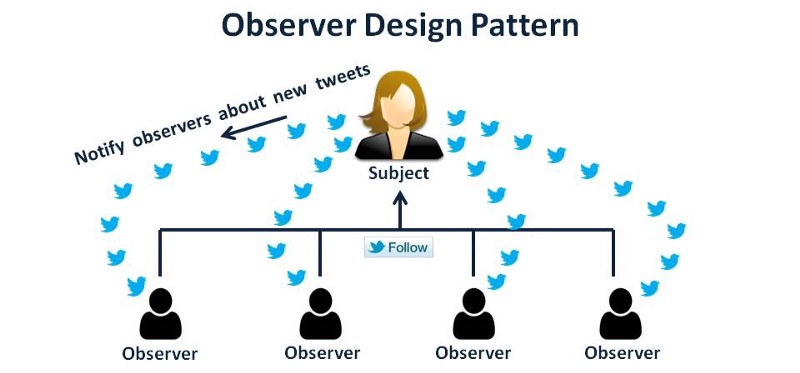
\includegraphics[width=\textwidth]{images/observerPattern.jpeg}
  
  Um der das Oberserver Pattern zu implementieren, wird ein Class \glqq Observable\grqq bei diesem Projekt erstellt.
  
  image: Observable .........
  
  Während der Erstellung einer Observable wird ein Array generiert, um die Observers zu speichern. Durch die Funktionen subscribe und unsubscribe können die Observers in dem Array eingefügt oder von dem Array ausgezogen werden. Die Observers(Funktionen) sollen ein Parameter haben, um die Nachrichten von Observer zu empfangen. Wenn die Funktion Notify aufgerufen wird, werden alle Observers in dem Array nacheinander aufgerufen. Der Parameter der Funktion Notify wird als Parameter der Observers eingesetzt, sodass die Nachrichten auszuteilen.
  
  
  \subsubsection{Zustände Management}
  
  Um das Zustand Management zu realisieren, wird ein Class stateIndex geschrieben. Da fast alle Objekt in der Szene mit diesem Class verbinden und das einzige \glqq state container\grqq referenzieren, wird das Class als \glqq static\grqq Class definiert.
  
  Mit init Funktion werden alle Zustände initialisiert. Die Initialisierung liegt an dem Query string in URL. Das Query string ist ein Teil von URL, dadurch der  Parameter bei dem \glqq request\grqq zusammen an dem Server geschickt. Bei dieser Applikation soll das Query string die Ziffer des ausgewählten Abschnitt sein. Mit dem Query string wird die Zustände nach dem Ausgewählten Abschnitt initialisiert.
  
  Während der Initialisierung wird eine Entität von Observable erstellt, um die Benachrichtigung vorzubereiten.
  
  Die init Funktion wird nur ein mal durchgeführt, wenn die Applikation aufgerufen.
  
  image: URL mit Query string .........
  
  Zu Sichert darf die Zustände von andere Objekt nicht erreichen. Deswegen werden die Funktionen von Class stateIndex angeboten, um die Zustände zu manipulieren.
  
  \begin{itemize}
      \item \textbf{getState}: alle aktuelle Zustände zu bekommen.
      \item \textbf{get}: bestimmte Zustand zu bekommen.
      \item \textbf{getIn}: bestimmte Zustand in tiefen Ebenen zu bekommen.
      \item \textbf{set}: bestimmte Zustand zu aktualisieren. Durch der Funktion Notify von Observable die neue Zustände an allen Observer auszuteilen.
      \item \textbf{setIn}: bestimmte Zustand in tiefen Ebenen zu aktualisieren. Durch der Funktion Notify von Observable die neue Zustände an allen Observer auszuteilen.
  \end{itemize}
  
 \subsection{Abschnitte Auswahl}

 Der Auswahl der Abschnitte kann auf zwei Zeitpunkten durchgeführt werden. Einer davon ist während der Aufruf der Applikation. Die Ziffer der ausgewählte abschnitt wird durch dem Query string in URL an der Applikation gegeben. Der andere ist vor dem Nahm der Krankenakte in VR Szene. Auf dem Whiteboard werden die Abschnitte aufgelistet, dadurch bestimmter Abschnitt auswählen werden kann.
 
  \subsubsection{Abschnitte Auswahl durch URL}
  Die Zustände werden am Anfang als ursprüngliche Zustände initialisiert. Durch der Funktion getSectionSelectionFromURL in Class stateIndex kann die ausgewählte Ziffer bestimmen werden. Wenn die Ziffer zwischen 1 und 7 ist, werden die betreffende Zustände durch die Funktion selectSection aktualisiert. Danach werden die Objekte in der Szene nach den Zuständen auch aktualisiert.
  
  Um die GUI richtig einzusetzen, wird ein Trick benutzt. Wenn die Applikation aufgerufen, wird die Szene nach den aktuellen Zuständen eingerichtet und werden gleichzeitig die Modells geladen. Es könnte passieren, dass das Modell noch nicht fertig geladen ist, wenn es von der Aktualisierung betroffen wird. Das führ zu Fehler der Applikation.
  
  Um das Problem zu lösen, werden die Ladung vor der Aktualisierung überprüft. Mit der Funktion setInterval wird es implementiert, jede 0,5 Sekunde die Zustand der Ladung zu überprüfen. Wenn alle Modells schon geladen ist, wird die Überprüfung beendet und die Szene aktualisiert.
  
  image: Überprüfen die Ladung .........
  
  \subsubsection{Abschnitte Auswahl in VR Szene}
  Auf dem Whiteboard wird die Abschnitte aufgelistet. Durch Zeiger oder Raycaster wird die Funktion selectSection in Class stateIndex mit entsprechendem Parameter aufgerufen, um der Abschnitt zu wechseln.
  
  Vor den Zeichnen auf dem Whitebard werden 7 \glqq toggle box\grqq eingesetzt, dadurch die Funktion selectSection von HTC Vive Controller aufgerufen kann.
  
  image: toggle box für Abschnitt .........
  
  \subsubsection{Verbesserung}
  Der Abschnitte Auswahl kann nicht nur während der Initialisierung, sondern auch nach der Initialisierung durchgeführt wird. Deswegen sollen die Funktionen über Abschnitte Auswahl wie selectSection nicht in Class stateIndex eingepackt werden, sondern in eigenen Datei geschrieben werden.
  
 \subsection{Gemeinsame Class Struktur der Objekten}
 Um effizient zu entwickeln 
 
 \subsection{Interaktion}
  \subsubsection{PC und Smartphone}
  \subsubsection{Samsung Gear VR}
  \subsubsection{HTC Vive}
 \subsection{Geräte anpassen}
 \subsection{Töne}
 \subsection{Uhr}
 \subsection{Hand}
 \subsection{Attribute Veränderung}
 
 \subsection{Arbeitsoberfläche Desinfektion in Vive}
 \subsection{Animation}
 \subsection{Kollision Erkennung}
 \subsection{Transparenz}
 \subsection{Fallen}


